\paragraph{QuizziPedia::Back-End::App::Models::LangModel}
\label{QuizziPedia::Back-End::App::Models::LangModel}
\begin{figure}[ht]
	\centering
	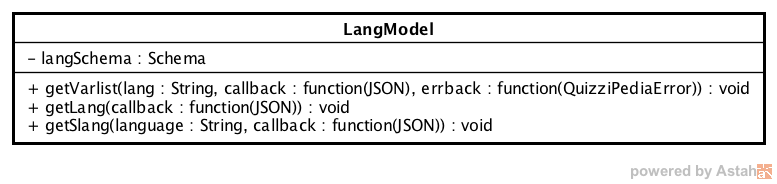
\includegraphics[scale=0.8]{UML/Classi/Back-End/QuizziPedia_Back-End_App_Models_langModel.png}
	\caption{QuizziPedia::Back-End::App::Models::LangModel}
\end{figure}
\FloatBarrier
	\begin{itemize}
		\item \textbf{Descrizione}: classe che modella le informazioni riguardanti la lingua dell'applicazione;
		\item \textbf{Utilizzo}: viene utilizzata per scambiare memorizzare le traduzioni delle variabili che andranno visualizzate nella \textit{view\ped{G}};
		\item \textbf{Relazioni con altre classi}:
			\begin{itemize}
				\item \textbf{OUT \texttt{LangController}} \\
				Classe che gestisce la logica applicativa riguardante la traduzione delle variabili.
			\end{itemize}
		\item \textbf{Attributi}:
			\begin{itemize}
				\item \texttt{LangSchema : Schema} \\
				Questo campo rappresenta lo schema \textit{mongoose\ped{G}} per le variabili della lingua e prevede i seguenti attributi:
					\begin{itemize}
						\item \texttt{lang: String}, rappresenta la lingua scelta per l'applicazione;
						\item \texttt{variables: Array<String>}\\ Array associativo che contiene delle \texttt{String} necessarie per la giusta traduzione dell'applicazione.
					\end{itemize}
			\end{itemize}
		\item \textbf{Metodi}:
			\begin{itemize}
				\item \texttt{+ getVarlist(lang: String, callback: function(JSON)): void} \\
				Metodo che permette di ritornare la traduzione delle variabili. \\
				\textbf{Parametri}:
					\begin{itemize}
						\item \texttt{lang: String} \\
						Rappresenta l'informazione che indica il set di traduzione da ritornare;
						\item \texttt{callback: function(JSON)} \\
						Rappresenta la \textit{callback\ped{G}} che verrà eseguita al termine dell'elaborazione nel caso non si verifichino errori durante l'esecuzione;
					\end{itemize}
				\item \texttt{+ getLang(callback: function(JSON)): void} \\
				Metodo che permette di ritornare un array di variabili che serviranno per la traduzione \\
					\textbf{Parametri}:
					\begin{itemize}
						\item \texttt{callback: function(JSON)} \\
						Rappresenta la \textit{callback\ped{G}} che verrà eseguita al termine dell'elaborazione nel caso non si verifichino errori durante l'esecuzione;
					\end{itemize}	
				\item \texttt{+ getSlang(llanguage:String,callback: function(JSON)): void} \\
				Metodo che permette di ritornare un array di variabili che serviranno per la traduzione \\
					\textbf{Parametri}:
					\begin{itemize}
							\item \texttt{language: String} \\
							Rappresenta l'informazione che indica il set di traduzione da ritornare;
							\item \texttt{callback: function(JSON)} \\
							Rappresenta la \textit{callback\ped{G}} che verrà eseguita al termine dell'elaborazione nel caso non si verifichino errori durante l'esecuzione;
					\end{itemize}	
			\end{itemize}
	\end{itemize}
	